\chapter{Multi-Faceted Evaluation}
The basic structure for faceted evaluation for dynamic information flow is as shown in Figure 1. This language is an extension of $\lambda$ -calculus with a special value called $\bot$ and facilities for creating faceted values. These semantics were developed as a part of previous work ~\cite{bib4}. This paper provides an implementation for the same in JavaScript that was discussed in previous paper, further checks for different possibilities of attacks that can be avoided. 

As shown in Figure 1, this language captures most of the essential features of dynamic information flow in many realistic languages. The language includes few of the key challenges like higher order function calls, implicit flows and mutable references. 

$\lambda^{facet}$ contains the following standard features like variables (x), functions ($\lambda_{x.e}$), function application ($e_{1}$, $e_{2}$) and constants (c). This language also supports referencing (ref e) and dereferencing (!e) and updating ($e_{1}$:= $e_{2}$) a reference cell. In order to model the same interactive nature of JavaScript, our $\lambda^{facet}$ also supports reading from and writing to files. The expression 
$$
<\ k\ ?\ e_{1}\ :\ e_{2}\ >
$$
is a faceted value, which says $e_{1}$ is a value that can only be observed by the private users. That is, if a user does not have access to the secret value, then he can only see the public value $e_{2}$.

The $\bot$ value that is shown in the language semantics above is a substitute for "nothing" , similar to null in Java or undefined in JavaScript. It is generally used as a public value with nothing to display as shown below. Where V denotes the private value. 
$$
<\ k\ ?\ V\ :\ \bot>
$$

\begin{figure}
\centering
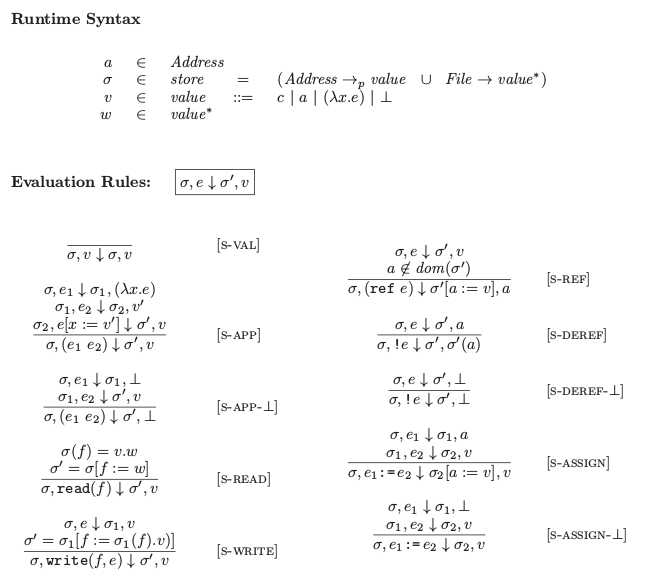
\includegraphics[width=1\textwidth]{images/fig2.png}
\caption[Standard Semantics.]{Standard Semantics. \\Source: ~\cite{bib4} } 
\label{fig:Source_semantics}
\end{figure}

Figure ~\ref{fig:Source_semantics} shows the standard semantics without faceted values. Values may be addresses, $\bot$ , constants or closures as shown. The store $\sigma_{}$ maps addresses to values and also files {\it f} to sequence of values {\it w}, each address is allocated to a reference cell a.

The standard semantics as shown in Figure ~\ref{fig:Source_semantics} can be interpreted as an expression e  
$$
\sigma ,e \downarrow \sigma^{'} ,v 
$$
in the context of store $\sigma_{}$ is evaluated, which results in a value v and the store $\sigma^{'}$ . To show one example, the rule [\ s-app\ ] evaluates the function body e which is called; the notation e[x\ :=\ v] says that it maps x to v for all values within expression e.

\begin{figure}
\centering
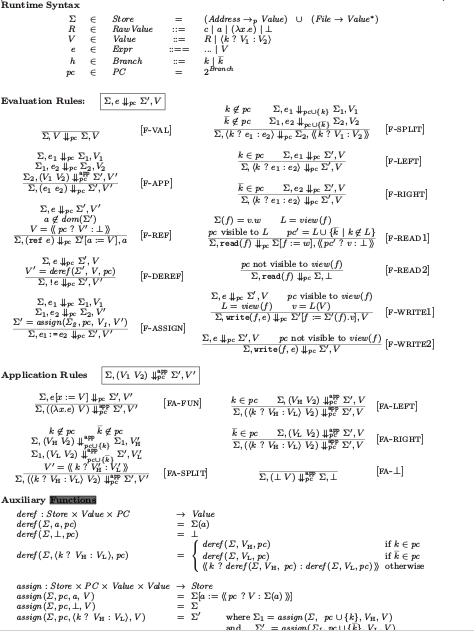
\includegraphics[width=0.90\textwidth]{images/fig7.png}
\caption[Extended Semantics with faceted values.]{Extended Semantics with faceted values. \\Source: ~\cite{bib4} } 
\label{fig:ExtendedSource_semantics_facetV}
\end{figure}

One unusual thing that can be observed here is the value $\bot$. Operations that include this are very strict in nature. Strict operations with $\bot$ clearly considers it as no value. This is different from having "undefined". We can see more on this when this is used as a part of faceted value
 
\section{Programming Constructs with Facets}
As the standard semantics are now defined, we now look into the extended semantics with faceted values that track information flow dynamically and provide non-interference
guarantees.

Figure ~\ref{fig:ExtendedSource_semantics_facetV} shows the additional runtime syntax that is required to support faceted values. Values "V" now contain faceted values of the form
$$
<\ k\ ?\ V_{H}\ :\ V_{L}\ >
$$
where $V_{H}$ is private facet and $V_{L}$ is public. The value 
$$
<\ k\ ?\ "Password"\ :\ \bot> 
$$
says that Password is confidential and can only seen by the user who has access to k.
NULL on the other side is viewed by unauthorized viewers.

A new label called the program counter(pc) is introduced to keep track of when program is influenced by public or private facets.
	
\section{Faceted Evaluation with Exceptions}
In this paper I have concentrated on providing exception support for faceted evaluation. If an exception is thrown due to a single facet of a faceted value, that must not be visible to unauthorized principals. JavaScript supports exceptions to smoothly handle errors. These exceptions introduce additional challenges to our analysis on evaluation with faceted values, as some branches of a faceted execution could terminate normally but others might throw exceptions.

\begin{figure}
\centering
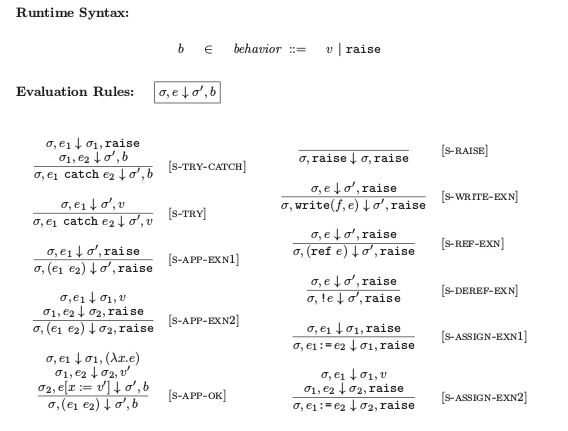
\includegraphics[width=0.85\textwidth]{images/fig3.png}
\caption[The Standard semantics to handle exceptions.]{The standard semantics to handle exceptions. \\ Source:  ~\cite{bib4}} 
\label{fig:exception_semantics}
\end{figure}

Thus, there is a need to extend our analysis to handles such cases like throwing and catching exceptions. We improve the syntax of $\lambda^{facet}$ as follows:
$$
	e ::= ...\ |\ raise\ |\ e_{1}\ catch\ e_{2}
$$	
Figure ~\ref{fig:exception_semantics} shows some of the additional rules for the standard semantics to handle exceptions. Unlike the normal standard semantics, an evaluation returns a behaviour (b), which can either be a value (v) or raise, marking an exception. We can describe [s-try-catch] rule as in an expression $e_{1}$ catch $e_{2}$, if $e_{1}$ is evaluated to raise, then $e_{2}$ is evaluated and the result is returned. Otherwise, $e_{1}$ is evaluated and the result is returned.

\begin{figure}
\centering
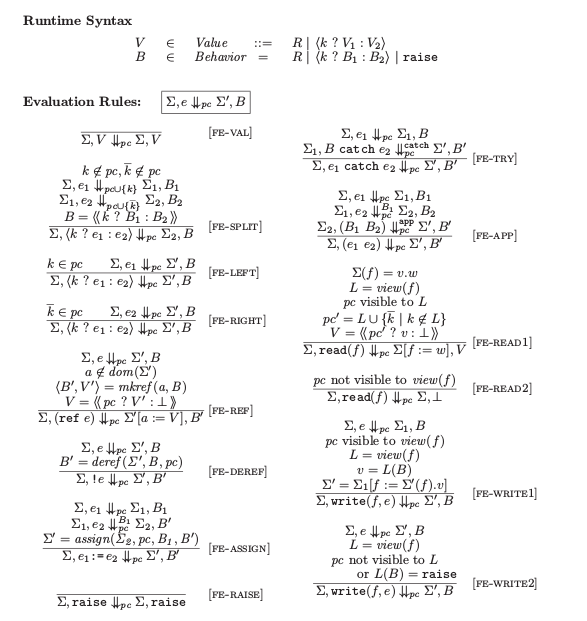
\includegraphics[width=0.85\textwidth]{images/fig4.png}
\caption[Core rules for Faceted Evaluation with Exception Handling.]{Core rules for Faceted Evaluation with Exception Handling. \\Source: ~\cite{bib4}} 
\label{fig:core_FEEXH}
\end{figure}

\section{Faceted Exceptions}

\begin{figure}
\centering
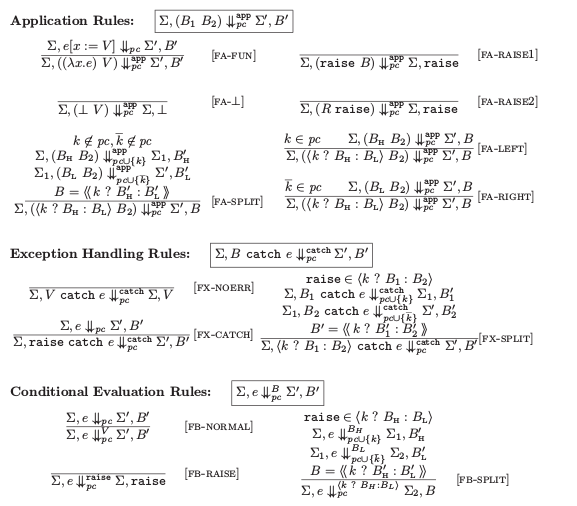
\includegraphics[width=0.85\textwidth]{images/fig5.png}
\caption[Faceted Evaluation Rules for Application and Exceptions.]
{Faceted Evaluation Rules for Application and Exceptions. \\Source: ~\cite{bib4} } 
\label{fig:FE_AEX}
\end{figure}
We now move a step forward and work on core rules for faceted evaluation with exceptions. Exception handling with faceted values requires considerable amount of care. As shown in Figure ~\ref{fig:core_FEEXH}, in an application ($e_{1}$ \ $e_{2}$), if $e_{1}$ evaluates to raise for some view of the faceted value, then $e_{2}$ should not be evaluated for that view. Similarly, an exception handling block should only be executed for views that witness an exception. In previous paper by Austin and Flanagan ~\cite{bib4}, there are two additional evaluation relations introduced to handle exceptions properly. The rules are further updated and presented in  Figure ~\ref{fig:FE_AEX}.

An additional evaluation relation has been introduced in the paper by Austin and Flanagan ~\cite{bib4}
$$
\sigma e  \downarrow \downarrow^{B}_{PC} \sigma^{'} B^{'}
$$
Here the evaluation of e is controlled by superscript B , so that this relation evaluates e only for views L for which L(B) not= raise: as shown in Figure ~\ref{fig:FE_AEX}. This says that e is evaluated normally if the observed behaviour B is a value, as mentioned by [fb-normal]. In other case, if B is raise, e is not evaluated and instead raise is returned as mentioned by [fb-raise]. The rule [fb-split] says that its called recursively on every facet when B is a faceted behaviour

An important property that has to be observed here is that if there is an exception that is raised for a particular view, this view will not be affected by the code part that has been skipped over due to an exception.